% ***** Класс ***** %
\documentclass[pdftex, a4paper, 14pt]{extreport} 

% ***** Файлы стилей ***** %
\usepackage{./STYLE/style}
\usepackage{./STYLE/styleCode}

% =================================================
% НАЧАЛО ДОКУМЕНТА
% =================================================
\begin{document}

% ***** Титульный лист ***** %
\import{TITLE/}{title} 

\section*{Цель работы}
Изучить материал и научиться находить решение в нелинейных обратных задачах.

\section*{Задание (Вариант 3)}
Положение приемников:
\begin{center}
    M1(200,0,0), N1(300,0,0); \\
    M2(500,0,0), N2(600,0,0); \\
    M3(1000,0,0), N3(1100,0,0). \\
\end{center}

Положение источников:
\begin{center}
    A1(0,-500,0), B1(100,-500,0); \\
    A2(0,0,0), B2(100,0,0); \\
    A3(0,500,0), B3(100,500,0). \\
\end{center}

Однородное полупространство. Приёмники 1–3. Источник 2. 
Определить значение $\sigma$ полупространства. Добавить шум, равный
10\% от значения измерения. 

\section*{Теория}
Формула связи электрического тока в источнике и напряжения в приёмнике:

\begin{equation*}
    V_{AB}^{MN} = \frac{I}{2\pi\sigma} \parens{\parens{\frac{1}{r_B^M} - \frac{1}{r_A^M}} - \parens{\frac{1}{r_B^N} - \frac{1}{r_A^N}}}
\end{equation*}

Производная потенциала по силе тока:
\begin{equation*}
    \parder{V}{I} = -\frac{1}{2\pi\sigma^2} \parens{\parens{\frac{1}{r_B^M} - \frac{1}{r_A^M}} - \parens{\frac{1}{r_B^N} - \frac{1}{r_A^N}}}
\end{equation*}

Выходить из итерационного процесса будем по малости функционала:
\begin{equation*}
    \Phi\parens{\sigma} = \SUM_{i=1}^3\parens{\omega_i \cdot \parens{V_i\parens{\sigma} - \overline V_i}}^2
\end{equation*}

\section*{Тесты}
\subsection*{Тест №1 (Без шума)}

\begin{equation*}
\begin{cases}
    I = 1 \\
    \mtext{Шум} = 0\% \\
    \mtext{Начальная sigma} = 0,01 \\
    \mtext{Истинная sigma} = 0,1 \\
    \mtext{Точность} = 1e-7 \\
\end{cases}    
\end{equation*}    
\begin{figure}
    \centering
    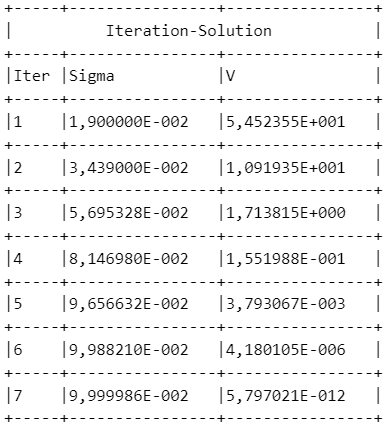
\includegraphics{IMG/NoNoise.png}
\end{figure}

\subsection*{Тест №2 (С шумом +10\%)}
\begin{equation*}
\begin{cases}
    I = 1 \\
    \mtext{Шум} = +10\% \\
    \mtext{Начальная sigma} = 0,01 \\
    \mtext{Истинная sigma} = 0,1 \\
    \mtext{Точность} = 1e-7 \\
\end{cases}    
\end{equation*}    
\begin{figure}
    \centering
    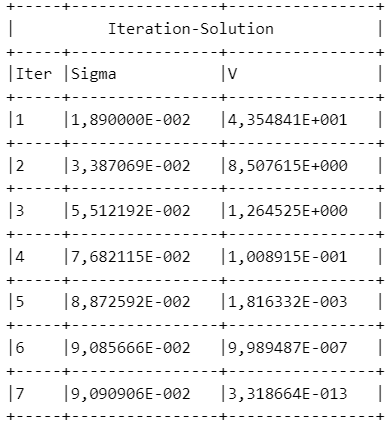
\includegraphics{IMG/YesPositiveNoise.png}
\end{figure}


\subsection*{Тест №3 (С шумом -10\%)}
\begin{equation*}
\begin{cases}
    I = 1 \\
    \mtext{Шум} = -10\% \\
    \mtext{Начальная sigma} = 0,01 \\
    \mtext{Истинная sigma} = 0,1 \\
    \mtext{Точность} = 1e-7 \\
\end{cases}    
\end{equation*}    
\begin{figure}
    \centering
    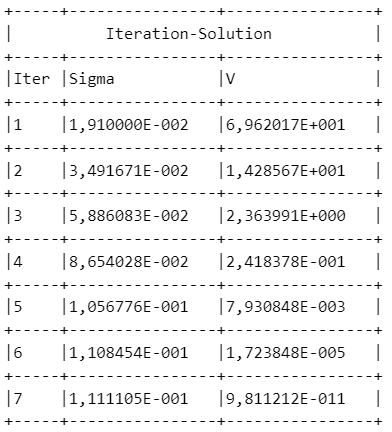
\includegraphics{IMG/YesNegativeNoise.png}
\end{figure}

\section*{Листинг}
\newpage

% ***** Program.cs ***** %
\begin{mybox}
    \begin{center}
        \textbf{Program.cs}
    \end{center}
\end{mybox}
\vspace{-8mm}
\inputminted
[ frame=lines,
  framesep=2mm,
  baselinestretch=1.2,
  bgcolor=LightGray,
  fontsize=\footnotesize,
  linenos,
  breaklines
]{csharp}{CODE/Program.cs}
% ******************************** %

% ***** Solve.cs ***** %
\begin{mybox}
    \begin{center}
        \textbf{Solve.cs}
    \end{center}
\end{mybox}
\vspace{-8mm}
\inputminted
[ frame=lines,
  framesep=2mm,
  baselinestretch=1.2,
  bgcolor=LightGray,
  fontsize=\footnotesize,
  linenos,
  breaklines
]{csharp}{CODE/Solve.cs}
% ******************************** %

% ***** Helper.cs ***** %
\begin{mybox}
    \begin{center}
        \textbf{Helper.cs}
    \end{center}
\end{mybox}
\vspace{-8mm}
\inputminted
[ frame=lines,
  framesep=2mm,
  baselinestretch=1.2,
  bgcolor=LightGray,
  fontsize=\footnotesize,
  linenos,
  breaklines
]{csharp}{CODE/Helper.cs}
% ******************************** %


\end{document}
% =================================================
% КОНЕЦ ДОКУМЕНТА
% =================================================